\documentclass[conference]{IEEEtran}
\usepackage{cite, graphicx}
\usepackage[utf8x]{inputenc}

\begin{document}
\title{Capturing Spending Trends with Venmo through Topic Modeling}

% author names and affiliations
\author{
\IEEEauthorblockN{Max Robinson}
\IEEEauthorblockA{Whiting School of Engineering \\ Johns Hopkins University\\
Baltimore, MD 21218\\
Email: Max.Robinson@jhu.edu}
}

% use for special paper notices
%\IEEEspecialpapernotice{(Invited Paper)}

% make the title area
\maketitle

% As a general rule, do not put math, special symbols or citations
% in the abstract
\begin{abstract}
Data on financial transactions is few and far between for public consumption. Trying to model or understand spending trends thus becomes a difficult task. However, a relatively new social media platform and financial transaction broker Venmo provides partial transaction data of users who wish to make transactions public. This paper finds that by using the information provided by users as part of the transaction, it is possible to generalize these transactions and discover spending trends over a period of time. 
\end{abstract}


\section{Introduction}
In a world where there is an explosion of data being produced and captured every day, it is surprisingly difficult to get publicly available financial data at the level of individual transactions. A large motivator for having these transactions is to use them to construct more general trends of how money gets spent over time. This information can then be used to make investment decisions, understand financial markets, and even understand behaviors. 

While financial data is collected and stored, it is usually closely guarded by banks and other financial brokers. Sample data does exist, but it is often old like that from the Prague Data Mining and Knowledge Discovery in Databases conference \cite{PKDD99} and may not be a good representation of current trends or markets. 

However, the popularity of social media sites has lead to the development and popularization of a particular peer to peer financial application called Venmo. Venmo is part social media platform, part financial broker. Venmo allows users to pay one another through their application. Users can also add messages as part of the transactions and the users can make these transactions public. 

The public data shown for the transaction includes the participants, the direction of the transaction, and the message sent with that transaction along with other metadata. This is the social media part of the application. Venmo provides a public API for any individual, to retrieve public transactions that have taken place using Venmo. 

As a result, Venmo has provided the public with a brand new source of financial data that was previously unobtainable. More than this, the data that is provided by Venmo is also likely to have ground truth about what the transaction was about, directly from the participant of the transaction. Given the messages are provided by the user, and that Venmo is a social media platform not dissimilar from other platforms like Twitter, similar challenges in understanding the text arise. 

This paper shows that given even a small amount of data, it is possible to generalize these transactions into topics. Once the topics have been found, it is shown that spending trends over time can be discovered and that these trends have a basis in reality. 

\section{Previous Work}
In order to gain generalized information out of collections of discrete objects, such as words, an idea of topic modeling was formed. One of the most popular topic modeling approaches currently is the latent Dirichlet allocation (LDA) \cite{LDA} model. LDA works by using a three-level hierarchical Bayesian model. This goal of the model is to approximate different topic probabilities for a given document. The topics with the highest probabilities are the topics that are most likely in the document. 

The domain of social media adds another layer of complexity into the world of text communication. Often times text on social media sites do not necessarily follow standard language grammar and often have variations of words or use additional characters such as emoticons or icons. 

Even with this added difficulty, LDAs have been applied to social media with quite a bit of success. LDA has been applied to different social media platforms such as Twitter \cite{EmpericalTopicTwitter} and even more specialized platforms like for avionics \cite{LDA-Avionics}.

Variations of LDAs have also been applied to social media, to try and tailor the LDA algorithm towards social media specific aspects. A variation that attempts to incorporate the temporal nature of social media data is TM-LDA \cite{TM-LDA}. TM-LDA works by attempting to learn the transition parameters among topics thus allowing it to identify when subsequent posts may not be part of the same topic. 

% to be replaced. 
%Previous work has be done on topic modeling with social media data, such as twitter. LDA has also been used in other places. 

%There is previous work done to model spending trends but this is mostly done with financial data, not social media data. 


\section{Experiment}
The goal of the experiment performed in this paper was to determine how groups of individuals are spending their money and if Venmo provides any insight into the trends of those spending habits. Each transaction in Venmo has the option to have a message associated with it. This message is filled in by the participant initiating the transaction. This information is what is collected and analyzed in the experiment. 

Since each transaction has a message, information has to be generalized and extracted across messages. To understand trends more generally, messages for the transactions in each day are generalized using Latent Dirichlet allocation (LDA) \cite{LDA} topic modeling. The topics and the words associated with that topic are then used to compare differences between days. These differences can then generalize to trends in the topics over time. 

\subsection{Data Collection}
Data was collected using Venmo's public web API. Data was collected for each day in April 2018, starting with April 1st and ending with April 30th. For each day, a random hour between the times of 08:00 and 23:00 EST was chosen to collect data for. About 600 records were then then collected from the time immediately prior to that hour. This results in about a 1 to 2 minute window of transactions being collected. So for example, if 09:00 was selected as the hour for collection, data was collected from about 08:57 to 08:59. 

Data was collected in this fashion due to some of the limitations of Venmo's public API. The public api does not allow for exact time queries, and has limits on the amount of data that is returned per query. To ensure that the experiment the procedure for using the API was to make an initial query for the hour selected, and then follow the API's ``next'' field, which specified the next URL to receive the next set of records. The initial query, and the number of times following the ``next'' totaled to 30 queries to the Venmo API for each day. 

The hour of day used to collect data was chosen at random. This was done to avoid biasing the data that was collected. Sampling hours randomly helps to decouple the time of day a transaction might take place with when in the month the transaction took place. The hours were limited to between 08:00 am and 23:00 EST. This was in an attempt to collect data during the times where the most number of transactions are suspected to take place. By collecting when more people are creating transactions, the data collected is more likely to be more diverse. 

For each day, roughly 600 transaction records were collected for analysis. This number of records was chosen in order to make the computation time, and collection times feasible for replication by many. Processing large amounts of data was not the goal of this experiment, thus about 600 records was settled on heuristically. In total, about 18,000 records were collected.

\subsection{Analysis}
The messages in the data collected is an unstructured text field that users are allowed to put any text they wish in. As a result, there is the opportunity for users to put all manner of messages or text in the field. In addition, since the message is for a financial transactions, many users put messages relevant to the transaction. This allows for the extracting of interesting information from messages. 

In order to understand all the transactions for a given day in a more general light, topic modeling is applied using Latent Dirichlet allocation (LDA) \cite{LDA}. Prior to generating the topics, the messages were preprocessed. The preprocessing is necessary to remove unwanted meaningless words from the messages.

\begin{figure}[!t]
  \centering
  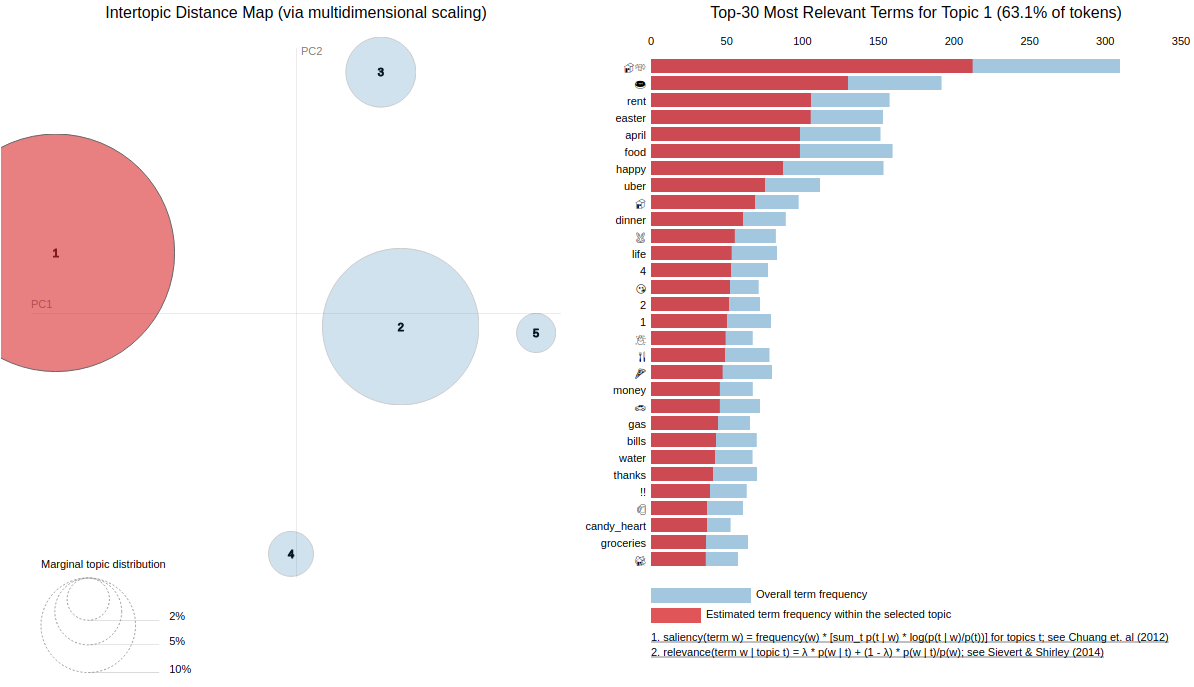
\includegraphics[width=\linewidth]{ldaVisTopics}
  \caption{LDA Visualization of topic distances from each other for data collected for April 1st using pyLDAvis}
  \label{fig:LDA-Distance}
\end{figure}

To preprocess the messages, the python Natural Language Toolkit (NLTK) \cite{NLTK} was leveraged. Messages were first tokenized according to NLTK's word punctuation tokenization. All English stop words that are apart of NLTK were removed from the messages. Additional punctuation tokens such as ?, \&, `,' , and ! were also included as stop words. 

Once the data was preprocessed, all of the words for a single day were used as the dictionary and corpus for LDA. An LDA model was built on this corpus. The model generated 5 topics for each day. The number of topics was selected after exploration of the collected data. It was found that 5 topics generated provided well separated topics without reducing any topic to containing non-relevant words. Figure \ref{fig:LDA-Distance} shows a plot of 5 topics using data collected for April 1st. The plot is generated using pyLDA \cite{pyLDA}, which is based on LDAvis \cite{LDAvis}.

Each topic consisted of 10 top words. The words also have varying relevance to the topic in importance from 1 to 10, 1 being most relevant and 10 being least relevant. This relates to the LDA coefficients for each word. Typically the first topic produced by LDA is the most encompassing topic when comparing to words frequency in the corpus. As such, the first topic will be used as a bellwether in this paper. 

% start to talk about how the results were analyzed. 
Two approaches were taken to analyze the resulting topics for each day. First was to look at the number of unique words across all of the topics for a given day and calculate how many words were the same from day to day. This is then compared to the number of unique words associated with the topics for that day. This shows if the words being used in the topics change over time. 

\begin{figure*}[!t]
  \centering
  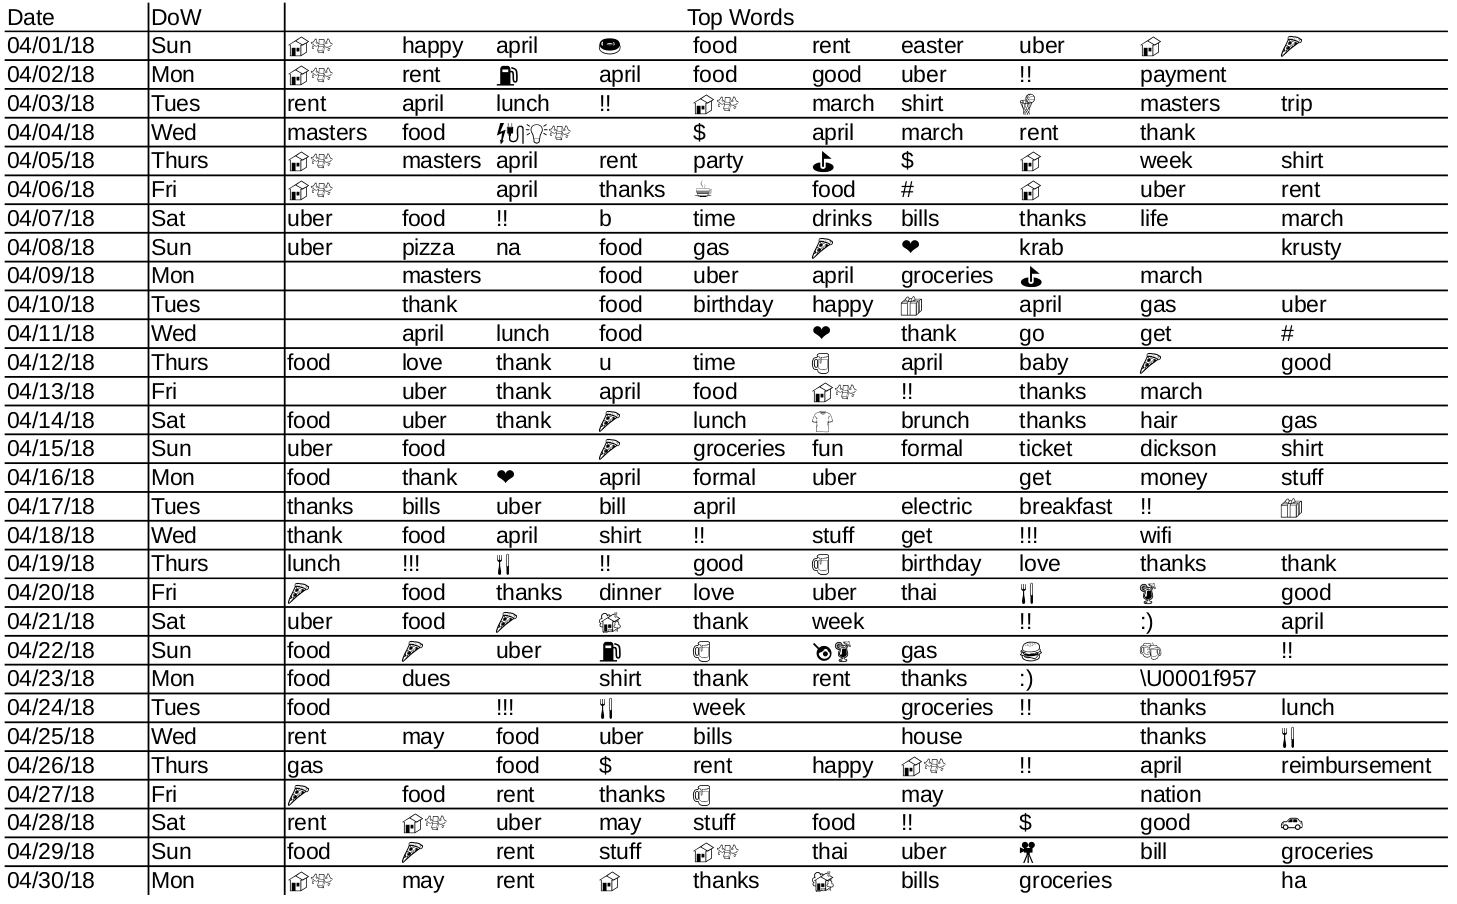
\includegraphics[width=0.8\textwidth]{Topic0FromDayToDay}
  \caption{Top Words in Topic 1 for each day in April 2018, with the most relevant words to the topic on the left and less relevant terms moving to the right.}
  \label{fig:Topic0FromDayToDay}
\end{figure*}

% results were analyzed by plotting the union of the unique word sets over time, compared to the number of words for that day.
The power of this comparison comes in trying to quantify if the topics change from day to day, and how much the topics might change. If there is no change in the words associated with a topic from day one to day two, and from day two to day three, this likely indicates that either there is not enough data to properly identify trends, or that the platform is likely void of trends. If the number of words changes too much, it is likely that again there is maybe not enough data or that the data collected is too noisy. If the number of changes is too high, it could also indicate that the the platform does not relay trends over time but instead just provides more or less random or unique comments in each message. 

% results were also examined by hand by looking at the first topic for each day and seeing if any trends could be seen by a human. 
The second analysis approach taken was to examine the words associated with the topics and compare them to the words associated with topics through out the month by hand. This approach was taken because it can be difficult to draw general trends over time from the words in each topic and on what day they were associated with. Many current approaches such as term frequency-inverse document frequency (TFIDF) \cite{TFIDF} which is used to determine the importance of certain words in a document, does not take into account the temporal nature of the data. While this sort of approach could summarize important words associated throughout the month, it would not determine when the words were important. 

Humans, however, tend to be relatively good at spotting temporal trends in data, and making correlations with other information associated with the data. A human can more easily spot trends like a word showing up in a topic correlated to days in the month, say every two weeks, and days of the week, like Friday. The dataset being explored is also relatively small. This allows for human analysis to spot trends that might otherwise be difficult to discover.

\section{Results}
% What were the results. 
Both analytic approaches described above were applied to the topics generated for each day in April. First the change in the number and overlap of unique words from day to day is examined. 

Figure \ref{fig:UniqueWordsOverTime} shows the trend over time of the unique terms from all of the topics compared the the unique terms in common from the previous day. This visualization shows that there are roughly 15 unique words across the 5 topics on a given day. In addition, there are about 5 unique words that are in common from day to on average. This means that on average about one-third of the unique words remained the same between two days, while about two-thirds would change. This visualization demonstrates a good mix in the number of unique words that vary from day to day given the number of unique words for that day. 

\begin{figure}[!t]
  \centering
  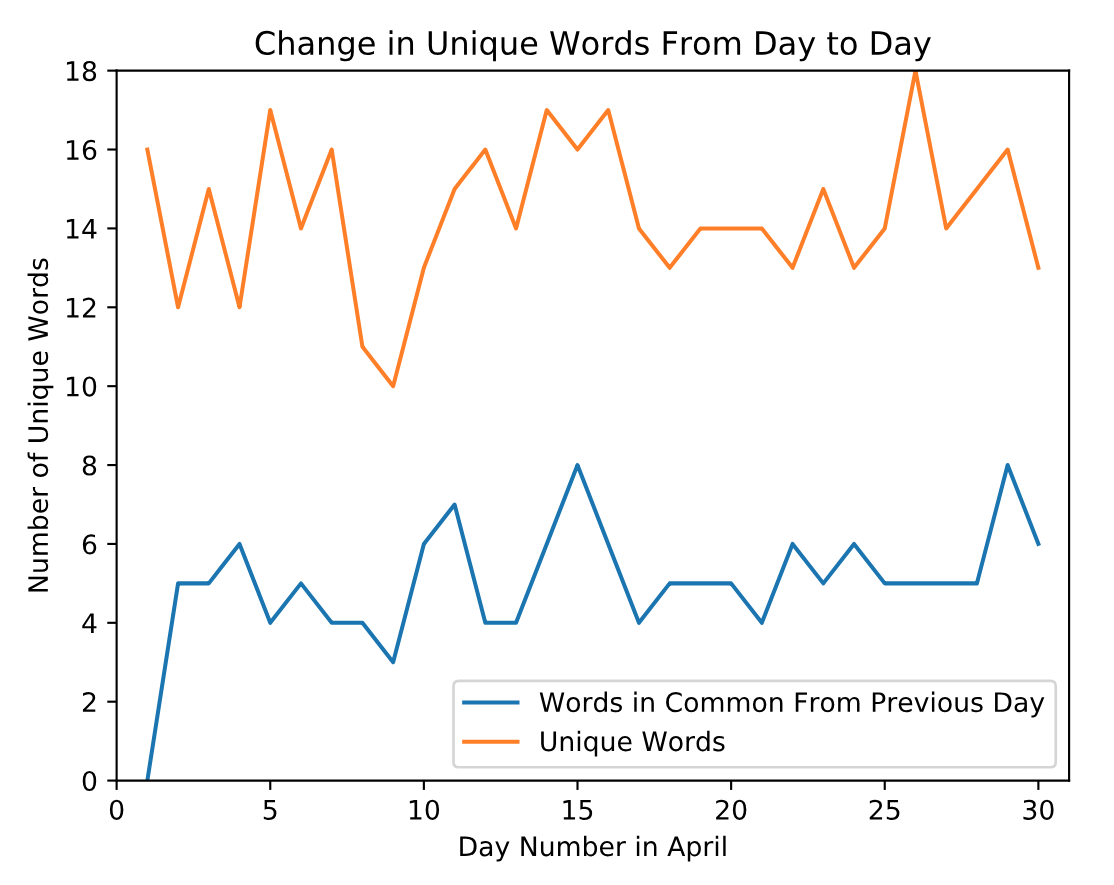
\includegraphics[width=0.9\linewidth]{UniqueWordsOverTime}
  \caption{Number of Unique words per day across all 5 topics for the day compared to the number of unique words across all 5 topics that were in common with the day previous to it.}
  \label{fig:UniqueWordsOverTime}
\end{figure}

This mix is quite important. If the number of words in common between days was a small percentage of the number of unique words for that day, this would indicate that trends over time would be unlikely. Conversely, if the percentage of unique words in common across days ways much higher, this would indicate that there were is only one trend, or a set of constant trends, which is not very interesting. Here we see that it is likely that there are at least words that are part of each days topics that are similar in following days, but also that there are parts that are different. This indicates that it is likely that there are at least trends lasting two or more days through out the month. 

The human analysis provides a deeper inspection of these likely trends and allows which trends are present to be identified. Figure \ref{fig:Topic0FromDayToDay} shows topic 1 for each day in April and the words associated with that topic. From this figure, trends in spending habits start to emerge. To analyze these possible trends, the words associated with the topics are correlated with the day of the month, the day of the week, and the words in the topics in days, as well as relevant context for that day. 

The first trend noticed is the prevalence of the house and flying money icons around the start of April. It is likely that transactions taking place have to do with rent or paying for something related to a house, like a mortgage. This is further supported by other words and symbols in the first week or so of April, like the dollar sign, house icon, and the word 'rent'. This would make sense as the first of the month is typically when rent or mortgage payments are due. This trend also emerges later in April towards the very end of the month, with similar characters and words to describe the trend. 

April 1st in 2018 was also Easter. This is also found to show up in this data through the words ``happy'' and ``easter'' in the topic for that day. These words do not show up together in any other days, but when correlated with the context for April 1st, these words associated with the topic is worth noticing. This gives confidence in the data and topic modeling that events outside of Venmo are being reflected in the trends. 

Other trends that become apparent are the type of services or items people spend money on at different points in the month. As the month progresses, more transactions tend towards things like goods, food, or Uber. For instance by April 9th food starts to show up as a more relevant term in the topics, suggesting that more transactions have to do with food as the month progresses. 

Another trend that can be observed are the transactions dealing with Uber. On weekends, it can be seen that the Uber jumps in relevance for the topics, but during the week the word almost disappears from the topics. This suggests that Uber is used mostly on weekends. Other trends such as when the beer or drink icons show up can also be correlated with the weekends. The combination of drinks and Ubers occurring on the weekends might be correlated, and might make common sense if individuals out drinking are avoiding drinking and driving. 

These trends seem quite grounded in both real world events and ``common knowledge'', such as when rent is due and avoiding drinking and driving. This provides a good foundation to believe that there is salient information in the messages provided with these transactions. This is necessary for believing identified trends that might not be as obviously grounded. An example might be looking at the trend for gas transactions. There is not a social consensus on when individuals buy gas, but gas seems to have its own trend.
%the other trends described help to validate that the trends that are not as well understood could be quite real and more believable.  

\section{Conclusion and Future Work}
This paper explored if information collected from Venmo could provide insight into spending trends over the course of time. Through the random sampling of data from Venmo, and applying topic modeling, evidence was provided that spending trends could be discovered, even with with small amounts of data. 

Correlating some trends with the time of the month, or day of the week also demonstrated that the trends observed make sense in a real world context. This provides the foundation to believe this approach can model real behaviors and trends. 

Some of the next steps to explore would be applying this results of this paper to a much larger set of data collected from Venmo. While a small amount of data showed trends, using a larger set of data would likely do better at modeling what a larger portion of the Venmo user community are spending their money on. 

As the amount of data increases, and the need for more topics per day is likely, ways to detect these trends over time and make associations between similar or semantically equivalent words will be much more necessary. Future work should focus on this trend detection. Likely some natural language processing will be needed. 

Lastly, Venmo provides near real time data. This enables future work to focus on how topics and spending trends can be found as the transactions occur.


% use section* for acknowledgment
%\section*{Acknowledgment}
%The authors would like to thank...



% An example of a floating figure using the graphicx package.
% Note that \label must occur AFTER (or within) \caption.
% For figures, \caption should occur after the \includegraphics.
% Note that IEEEtran v1.7 and later has special internal code that
% is designed to preserve the operation of \label within \caption
% even when the captionsoff option is in effect. However, because
% of issues like this, it may be the safest practice to put all your
% \label just after \caption rather than within \caption{}.
%
% Reminder: the "draftcls" or "draftclsnofoot", not "draft", class
% option should be used if it is desired that the figures are to be
% displayed while in draft mode.
%
%\begin{figure}[!t]
%\centering
%\includegraphics[width=2.5in]{myfigure}
% where an .eps filename suffix will be assumed under latex, 
% and a .pdf suffix will be assumed for pdflatex; or what has been declared
% via \DeclareGraphicsExtensions.
%\caption{Simulation results for the network.}
%\label{fig_sim}
%\end{figure}

% Note that IEEE typically puts floats only at the top, even when this
% results in a large percentage of a column being occupied by floats.


% An example of a double column floating figure using two subfigures.
% (The subfig.sty package must be loaded for this to work.)
% The subfigure \label commands are set within each subfloat command,
% and the \label for the overall figure must come after \caption.
% \hfil is used as a separator to get equal spacing.
% Watch out that the combined width of all the subfigures on a 
% line do not exceed the text width or a line break will occur.
%
%\begin{figure*}[!t]
%\centering
%\subfloat[Case I]{\includegraphics[width=2.5in]{box}%
%\label{fig_first_case}}
%\hfil
%\subfloat[Case II]{\includegraphics[width=2.5in]{box}%
%\label{fig_second_case}}
%\caption{Simulation results for the network.}
%\label{fig_sim}
%\end{figure*}
%
% Note that often IEEE papers with subfigures do not employ subfigure
% captions (using the optional argument to \subfloat[]), but instead will
% reference/describe all of them (a), (b), etc., within the main caption.
% Be aware that for subfig.sty to generate the (a), (b), etc., subfigure
% labels, the optional argument to \subfloat must be present. If a
% subcaption is not desired, just leave its contents blank,
% e.g., \subfloat[].


% An example of a floating table. Note that, for IEEE style tables, the
% \caption command should come BEFORE the table and, given that table
% captions serve much like titles, are usually capitalized except for words
% such as a, an, and, as, at, but, by, for, in, nor, of, on, or, the, to
% and up, which are usually not capitalized unless they are the first or
% last word of the caption. Table text will default to \footnotesize as
% IEEE normally uses this smaller font for tables.
% The \label must come after \caption as always.
%
%\begin{table}[!t]
%% increase table row spacing, adjust to taste
%\renewcommand{\arraystretch}{1.3}
% if using array.sty, it might be a good idea to tweak the value of
% \extrarowheight as needed to properly center the text within the cells
%\caption{An Example of a Table}
%\label{table_example}
%\centering
%% Some packages, such as MDW tools, offer better commands for making tables
%% than the plain LaTeX2e tabular which is used here.
%\begin{tabular}{|c||c|}
%\hline
%One & Two\\
%\hline
%Three & Four\\
%\hline
%\end{tabular}
%\end{table}


% Note that the IEEE does not put floats in the very first column
% - or typically anywhere on the first page for that matter. Also,
% in-text middle ("here") positioning is typically not used, but it
% is allowed and encouraged for Computer Society conferences (but
% not Computer Society journals). Most IEEE journals/conferences use
% top floats exclusively. 
% Note that, LaTeX2e, unlike IEEE journals/conferences, places
% footnotes above bottom floats. This can be corrected via the
% \fnbelowfloat command of the stfloats package.


% trigger a \newpage just before the given reference
% number - used to balance the columns on the last page
% adjust value as needed - may need to be readjusted if
% the document is modified later
% \IEEEtriggeratref{8}
% The "triggered" command can be changed if desired:
% \IEEEtriggercmd{\enlargethispage{-5in}}

% references section

% can use a bibliography generated by BibTeX as a .bbl file
% BibTeX documentation can be easily obtained at:
% http://www.ctan.org/tex-archive/biblio/bibtex/contrib/doc/
% The IEEEtran BibTeX style support page is at:
% http://www.michaelshell.org/tex/ieeetran/bibtex/
\bibliographystyle{IEEEtran}
\bibliography{IEEEabrv,VenmoTrends}


% that's all folks
\end{document}